\section{Background}
\label{sec:background}

To clarify the foundations in which this work relies, and to provide a starting 
point for understanding the rest of the thesis, this chapter introduces and 
describes two related and significant research motivations in which this dissertation is based. 
First, introducing our previous experience with \ac{aui} systems; and secondly, 
describing one of the basis that support the work described in this dissertation, 
which deals with the problem of identifying the user's disabilities and needs.

Consequently, Section~\ref{sec:background_imhotep} introduces Imhotep, an \ac{aui}
framework whose benefits and drawbacks have driven the research performed in this 
thesis. Next, in Section~\ref{sec:background_icf} \ac{icf} and the user capabilities 
related to interaction are addressed.

\subsection{Previous Experience with \acp{aui}: The Imhotep Framework}
\label{sec:background_imhotep}

Conceived in 2010, Imhotep~\citep{almeida_imhotep_2011} stands as the result of 
our first approach to \ac{aui} systems. Imhotep is a framework whose main goal
is to ease the development of adaptable and more accessible user interfaces. 
Designed by developers and \textit{for developers}, this framework allows
writing applications in a way in which developers do not have to worry about the 
adaptation of the user interface. The paradigm in which Imhotep is supported 
deals with the definition of a series of preprocessor directives. With these 
directives both the user capabilities and the device characteristics are taken
into account. 

To make the developed applications available to users, they are uploaded to 
a public repository. Thus, users can download them through an application 
download tool which sends to the server the user's and device's profile. Hence, 
the server compiles the best user interface for these profiles.

One of the benefits of Imhotep is the level of expression of the preprocessor
directives. Developers can establish their own variables and rules.
Listing~\ref{lst:imhotep_pseudocode} shows a piece of pseudo-code where the
developer defines new variables.

\inputminted[linenos=true, fontsize=\footnotesize, frame=lines]{java}{5_experiments_and_results/imhotep_pseudocode.txt}
\captionof{listing}{Imhotep pseudo-code defining variables~\citep{imhotep_website}.\label{lst:imhotep_pseudocode}}

These variables, rules and possible values are defined by the developer using a
web based wizard. Furthermore, the concepts, such as \textit{``resolution is 
big''} are created by the system taking into account the information of the mobile
devices (provided by \ac{wurfl}\footnote{http://wurfl.sourceforge.net/}) and pondering it with their 
popularity (with Google Trends\footnote{https://www.google.com/trends/} data).

The results obtained in Imhotep have motivated this dissertation. Moreover, Imhotep
serves as a good metric to evaluate the benefits of AdaptUI (the \ac{aui} platform 
described in this thesis). A more specific review of Imhotep is given in 
Chapter~\ref{cha:evaluation}, in which the Imhotep's architecture is reviewed 
and its performance compared with AdaptUI.


\subsection{User's Capabilities and Interaction}
\label{sec:background_icf}

Researchers have developed and improved several techniques to model users for 
the past 20 years~\citep{petrelli_user_centered_1999}~\citep{fink_adaptable_1997}. 
Modelling users implies gathering knowledge of their capabilities, drawbacks 
and limitations. During these first decades there was not any official and 
medical-based study to support user capabilities. Nevertheless, in 2001 
this situation changed. The \ac{wha}, a forum through which the \ac{who} is
governed, published the \ac{icf}\footnote{http://www.who.int/classifications/icf/en/}. 
\ac{icf} is a classification of human functioning and disability. It 
classifies every function state associated with health (e.g., diseases, 
disruptions, injuries and traumas). Its purpose is to identify the low-level 
capabilities relevant to product design in several domains. As was written by 
experts in the area, \ac{icf} is a reference for identifying several user 
capabilities in any interaction process. Its main goals are the following:

\begin{itemize}
  \item To provide a scientific basis to study and understand health and
  health-related states, outcomes and determinants.
  \item To establish a common language for describing health-related states in 
  order to improve communication between different users, such as health care 
  workers, researchers, policy-makers and the public, including people with 
  disabilities.
  \item To permit comparison of data across countries, health care disciplines,
  services and time.
  \item To provide a systematic coding scheme for health information systems.
\end{itemize}

\ac{icf} is organized into two main groups. On the one hand, Part 1 deals with 
\textit{Functioning and Disability}, indicating problems (e.g. impairment, 
activity limitation or participation restriction summarized under the umbrella 
term disability). On the other hand, Part 2 covers \textit{Contextual Factors}. 
This group gathers a list of \textit{Environmental Factors} which have an impact 
on all components of functioning and disability. The most significant function
groups of Part 1 are highlighted below:

\begin{itemize}
  \item \textit{Body functions}, which are the physiological functions of body 
  systems (including psychological functions). These functions encompass:
    \begin{itemize}
      \item Mental functions.
      \item \textit{Sensory functions and pain}.
      \item Voice and speech functions.
      \item \textit{Neuromusculoskeletal and movement-related functions}.
    \end{itemize}
  \item Body structures, as the anatomical parts of the body such as organs, 
  limbs and their components.
  \item Activities and participation. An activity is defined as the execution of 
  a task or action by an individual. Participation is involvement in a life 
  situation.
  \item Environmental factors, which make up the physical, social and attitudinal
  environment in which people live and conduct their lives.
\end{itemize}

In Part 2, \textit{Environmental factors} include:

\begin{itemize}
  \item Products and technology.
  \item \textit{Natural environment and human-made changes to environment.} It 
  encompasses:
  \begin{multicols}{2}
    \begin{itemize}
      \item Physical geography.
      \item Population.
      \item Flora and fauna.
      \item \textit{Climate}.
      \item Natural events.
      \item Human-caused events.
      \item \textit{Light}.
      \item \textit{Time-related changes}.
      \item \textit{Sound}.
      \item \textit{Vibration}.
      \item Air quality.
    \end{itemize}
  \end{multicols}

  \item Support and relationships.
  \item Attitudes.
  \item Services, systems and policies.
\end{itemize}

Two significant terms that this dissertation uses are \textit{impairment} and 
\textit{environmental factors}, defined by \ac{icf} as follows:

\begin{description}
  \item[\Defi{Impairments, by \ac{icf}}] \hfill \\
    \begin{mdframed}[hidealllines=true,backgroundcolor=gray!20]
    \textit{``Impairments are problems in body function or structure such as a 
    significant deviation or loss''.}
    \end{mdframed} 
    
  \item[\Defi{Environmental factors, by \ac{icf}}] \hfill \\
    \begin{mdframed}[hidealllines=true,backgroundcolor=gray!20]
    \textit{``Environmental factors make up the physical, social and attitudinal
    environment in which people live and conduct their lives''.}
    \end{mdframed} 
\end{description}

% First, the \textit{sensory functions} under the \textit{body functions} category of Part 1 are as the reference for adapting the user interface.

% This dissertation considers the function components remarked above. The 
% description of each component is detailed in Table~\ref{tbl:icf}.

\ac{icf} and its considerations, its mentioned and highlighted functions
classification support the motivation for this thesis.

\begin{table}
  \caption{\ac{icf} components considered in this dissertation.}
  \label{tbl:icf}
  \footnotesize
  \centering
  \begin{tabular}{l l l l}
    \hline
    \textbf{Category} 	& \textbf{Component group}& \textbf{Function}& \textbf{Description}\\
    \hline
    Body functions& Seeing and 	 	& Visual acuity	& Seeing functions of sensing from and	\\
    (Part I)	& related		& 		& contour, both binocular and monocular,\\
		& functions		& 		& for both distant and near vision.	\\
		& Hearing and 		& Hearing 	& Sensory functions relating to sensing \\
		& vestibular		& 		& the presence of sounds and discriminating\\
		& functions		& 		& the location, pitch, loudness and quality\\
		& 			&		& of sounds.				\\
		& Neuromusculos- 	& Mobility of 	& Functions of the range and ease of	\\ 
		& keletal and 		& a joint	& movement of a joint.			\\
		& movement-related 	& 		& 					\\
		& functions		&		&					\\
    \hline
    Natural 	& Climate		& Temperature	& Meteorological features and events, such\\
    environment & 			& Precipitation	& as the weather.			\\
    and human-	&			& Wind		& 					\\
    made changes& Natural events	& 		& Geographic and atmospheric changes that\\
    to environment& 			& 		& cause disruption in an individual's 	\\
    (Part II)	& 			& 		& physical environment.			\\
		& Light			& Intensity	& Level or amount of energy being emitted\\
		& 			& 		& by either a natural or an artificial 	\\
		& 			& 		& source of light.			\\
		& Time-related 		& 		& Natural, regular or predictable temporal\\
		& changes		& 		& change.				\\
		& Sound			& Intensity	& Level or volume of auditory phenomenon\\
		& 			& 		& determined by the amount of energy being\\
		& 			& 		& generated.\\
    \hline
  \end{tabular}
\end{table}


% Besides, in the field of adaptive user interfaces


% \ac{icf} provides a multi-perspective approach to the classification of functioning 
% and disability as an \textit{interactive} and \textit{evolutionary} process. It 
% provides the building blocks for users who wish to create models and study 
% different aspects of this process. The interaction of the components remarked by
% \ac{icf} are illustrated in Figure~\ref{fig:icf_interaction}.
% 
% \begin{figure}
% \centering
% 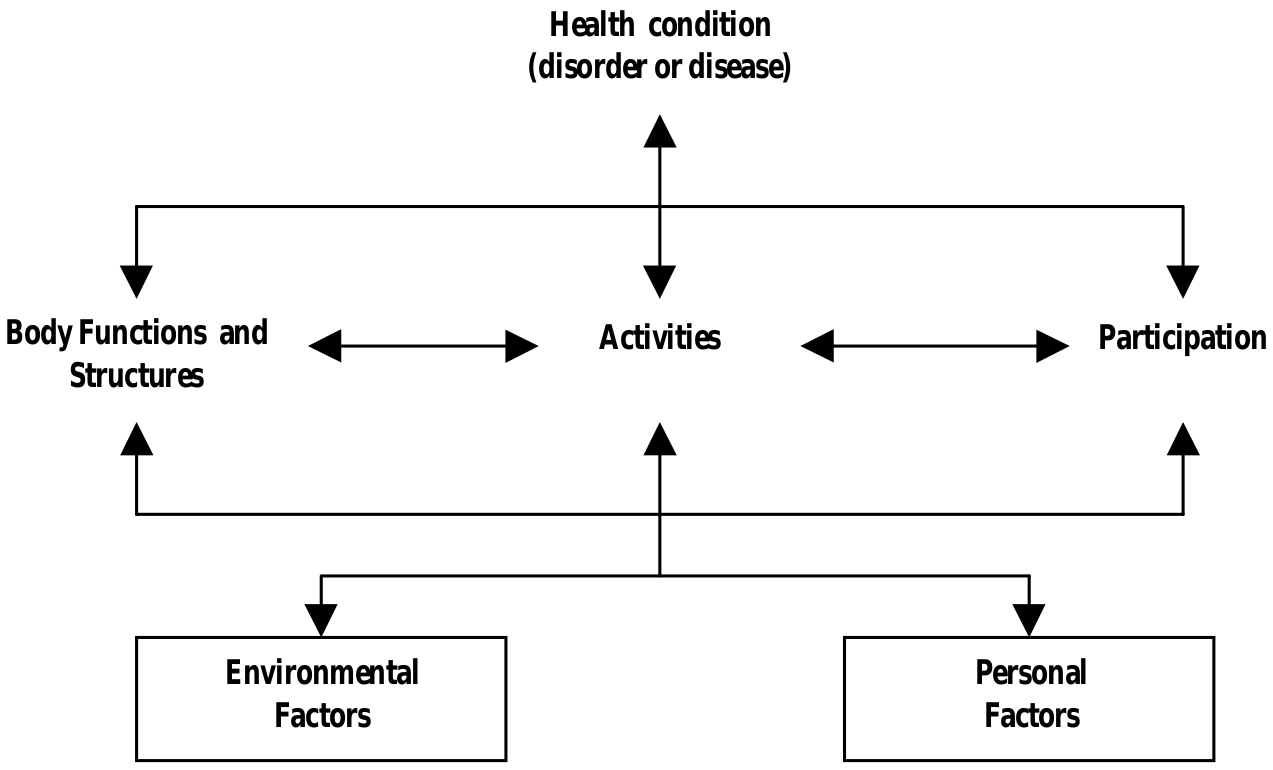
\includegraphics[width=0.75\textwidth]{icf_interaction.png}
% \caption{Interactions between the components of~\ac{icf}.}
% \label{fig:icf_interaction}
% \end{figure}